\documentclass{article}
\usepackage[utf8]{inputenc}
\usepackage[spanish]{babel}
\usepackage{listings}
\usepackage{graphicx}
\graphicspath{ {images/} }
\usepackage{cite}

\begin{document}

\begin{titlepage}
    \begin{center}
        \vspace*{1cm}
            
        \Huge
        \textbf{La memoria electrónica}
            
        \vspace{0.5cm}
        \LARGE
        Subtítulo
            
        \vspace{1.5cm}
            
        \textbf{Manuel Felipe Salazar Burgos}
            
        \vfill
            
        \vspace{0.8cm}
            
        \Large
        Despartamento de Ingeniería Electrónica y Telecomunicaciones\\
        Universidad de Antioquia\\
        Medellín\\
        Septiembre de 2020
            
    \end{center}
\end{titlepage}

\tableofcontents
\newpage
\section{Introducción}\label{intro}
A lo largo de los años, la tecnología a tomado gran importancia en la vida del ser humano, desde máquinas que realizaban el trabajo que podían hacer 20 hombres juntos en la época de la revolución industrial, hasta ordenadores que realizan multitud de tareas que son imposibles de procesar por un cerebro humano, en esta ocasión nos enfocaremos en estos ordenadores, y en específico en sus componentes, haciendo enfasis así en uno de sus "órganos" vitales, la memoria.

\section{La memoria, vital para un ordenador} \label{memory}
La memoria informática, o como coloquialmente se le llama, la memoria, se define como componente imprescindible del ordenador que mantiene disponibles las instrucciones para el microprocesador o CPU pueda ejecutarlas,\cite{https://www.ecured.cu/Memoria_(inform}, así, conociendo su definición, podemos conocer los tipos de memorias que hay, sus diferencias y sus labores en los ordenadores.
\subsection{Tipos de memoria}
En el hardware de una computadora podemos encontrar dos tipos de memoria, como lo son la memoria ROM y la memoria RAM; La memoria ROM, como lo dicen sus siglas en inglés "Read Only Memory", es la encargada estrictamente de la lectura de archivos en las computadoras, esta, posee la cualidad de que al apagar el ordenador sigue almacenando los archivos que se encontraran en ella. Por ejmplo, en esta encontramos el sistema operativo, todos nuestros documentos, fotos, programas, etc.
\begin{figure}[h]
    \centering
    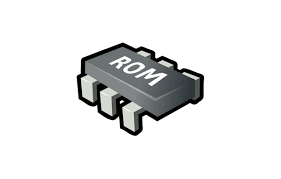
\includegraphics[width=6cm]{rom.png}
    \centering
    \caption{Memoria rom}
    \label{fig:memoryrom}
\end{figure} 
 Por otra parte, encontramos a la memoria ram "Random Access Memory", esta se encarga tanto de lectura como escritura en un lapso de tiempo temporal, es decir, al ser desconectada de una fuente de poder, pierde todos los datos que se encontraban almacenados en ella.
\begin{figure}[h]
    \centering
    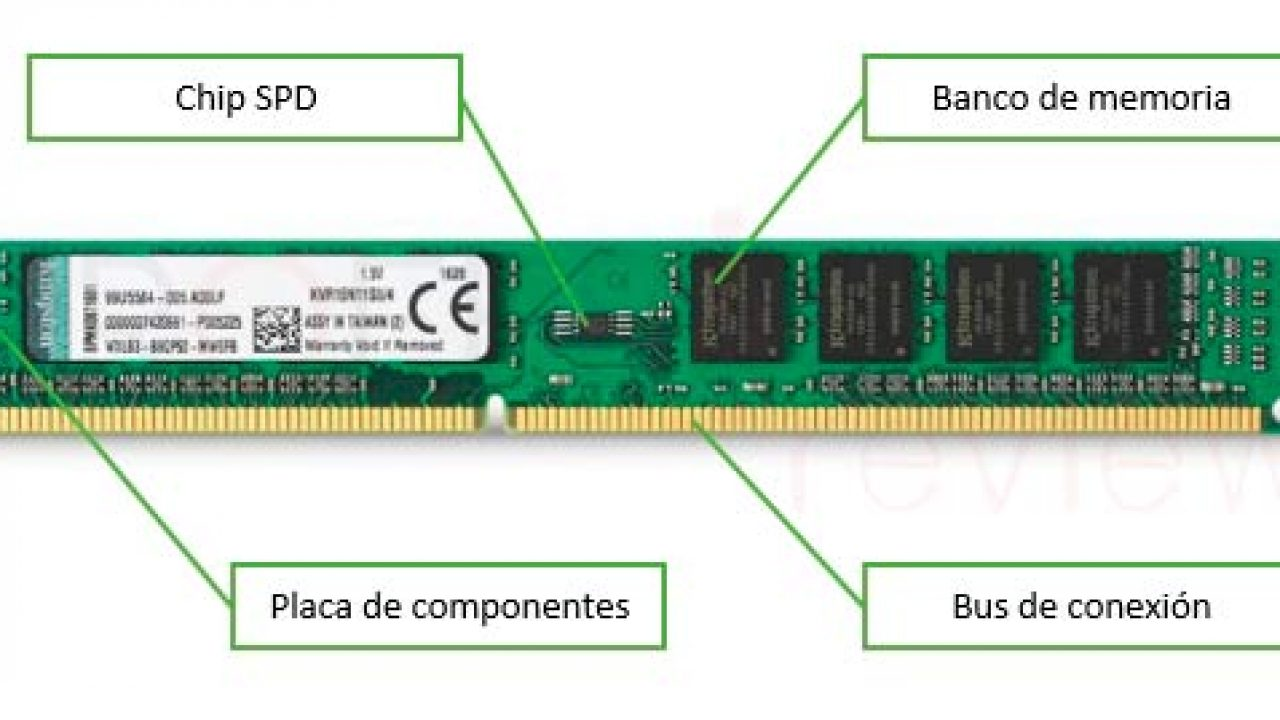
\includegraphics[width=6cm]{memory.jpg}
    \centering
    \caption{Memoria ram con sus partes}
    \label{fig:memoryram}
\end{figure} 
\section{Gestión de memoria en los ordenadores} 
La gestión de memoria en un ordenador, es fundamental para su funcionamiento, ya que esta se encarga de tanto entregar,como liberar la memoria que ya no se está usando en el sistema, el encargado de esto es el sistema operativo, así mismo se optimiza el uso de memoria para mejorar el rendimiento el las funciones del computador.
\section{Velocidad en las memorias} 
En los distintos tipos de memorias, existena unas que poseen más velocidad y por consiguiente mejor rendimiento que otras, por qué ocurrre esto?, desde un punto de vista más allá de la conductividad de los materiales con que se hacen estas, encontramos sus velocidades de lectura y escritura, lo cuál es vital, ya que entre mayor sean estas, más rapido se procesaran y leeran los archivos por el computador, otro aspecto que inlfuye en la memoria ram son los Mhz, los cuales se refieren directamente a su velocidad.


\bibliographystyle{IEEEtran}
\bibliography{references}

\end{document}
